
\titleformat{\chapter}
  {\gdef\chapterlabel{}
   \normalfont\sffamily\Huge\bfseries\scshape}
  {\gdef\chapterlabel{\thechapter\ }}{0pt}
  {
	\begin{tikzpicture}[remember picture,overlay]
	\node[yshift=-4cm] at (current page.north west)
	  {\begin{tikzpicture}[remember picture, overlay]
		\draw[fill=LightSkyBlue!20, draw=black, dashed] (0,0) rectangle
		  (\paperwidth,4cm);
		\node[anchor=east,xshift=.9\paperwidth,rectangle,
			  rounded corners=20pt,inner sep=11pt,draw,
			  fill=white, minimum width=6cm](name)
			  {  {\chapterlabel} \color{black}  #1   };
	   \end{tikzpicture}
	  };
   \end{tikzpicture}
   \vspace{2em}
  }




\usetikzlibrary{calc}
\title{
    \huge{\textcolor{blue}{Python 3与数据分析基础 \\---数据科学家的分析利器}} \\ ~ \\
	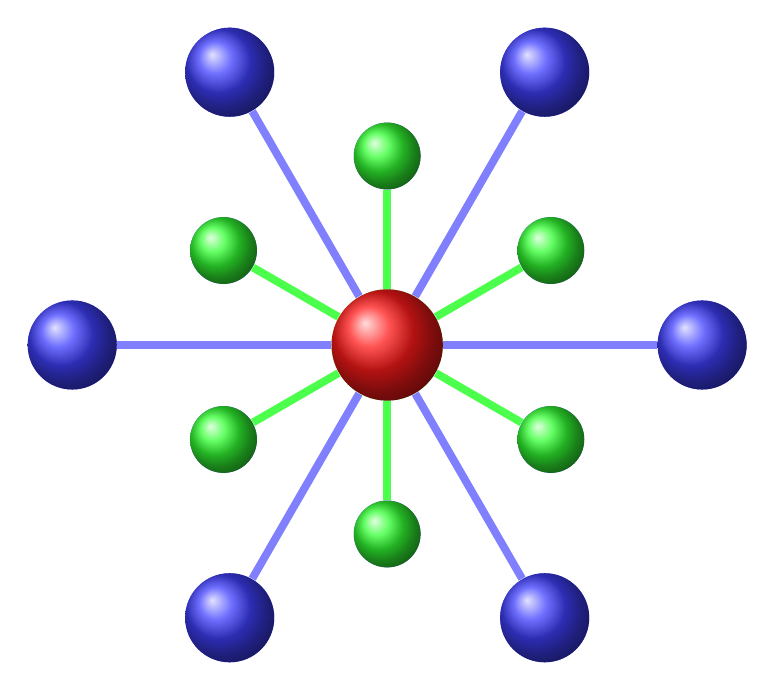
\begin{tikzpicture}
	\node[fill=green!60, shading=ball, ball color=red!90, shape=circle, inner sep=0.5cm] (0) {};
	\foreach \angle/\index in {0/1,60/2,120/3,180/4, 240/5, 300/6}{
		\node[fill=blue!60, shading=ball, ball color=blue!75, shape=circle, inner sep=0.4cm] (\index) at (\angle:4) {};
		\draw[line width=0.1cm, draw=blue!50] (0) to (\index);
	};
	\foreach \angle/\index in {30/1,90/2,150/3,210/4, 270/5, 330/6}{
		\node[fill=blue!60, shading=ball, ball color=green!80, shape=circle, inner sep=0.3cm] (\index) at (\angle:2.4) {};
		\draw[line width=0.1cm, draw=green!70] (0) to (\index);
	};
	\end{tikzpicture}
}
\author{
    夏天@IRM-Renmin University of China 
}

% General definitions for all Chapters
%-------------------------------------------------------------------------------
% Define Page style for all chapters


% Set double spacing for the text
\doublespacing
%-------------------------------------------------------------------------------


% 1st page for the Title
%-------------------------------------------------------------------------------
\maketitle

%-------------------------------------------------------------------------------
%用于生成罗马计数的前言
\frontmatter


